%TODO:
% Literaturzitate: \cite{bertsekas2007} % Gutes Lehrbuch etc.
% Edsger W. Dijkstra, 1959
% Nächste Schritte:
% Durcharbeiten Lattice CMU
% Kapiteleinteilung Unstrukturierte Umgebung
% Durcharbeiten Ziegler und McNorthon
% Kapiteleinteilung Strukturierte Umgebung

\chapter{Trajektorienoptimierung mittels Dynamischer Programmierung\index{Dynamische Programmierung}} \label{chap:dynamische_Optimierung_dynamisch}


\zitat{What title, what name, could I choose? In the first place I was interested in planning, in decision making, in thinking. But planning, is not a good word for various reasons. I decided therefore to use the word "`programming"'. I wanted to get across the idea that this was dynamic, this was multistage, this was time-varying. (\ldots) Thus, I thought dynamic programming was a good name.}{Richard E.\ Bellman }
 %It was something not even a Congressman could object to. So I used it as an umbrella for my activities.

Das Navigieren in einem Straßennetz, das automatisierte Anfahren einer engen Parklücke in mehreren Zügen und die Bestimmung der Ausweichrichtungen eines automatischen Kollisionsvermeidungsmanövers inmitten dynamischer Hindernisse sind Optimalsteuerungsprobleme\index{Optimalsteuerung} mit einer \emph{kombinatorischen} Note. Falls sich die Systemdynamik des jeweiligen Kernproblems auf \emph{wenige Zustände} beschränken lässt, dann besteht die Chance, das Problem als einen mehrstufigen Entscheidungsprozess formulieren zu können und es auf Basis der \emph{Dynamischen Programmierung} zur Laufzeit zu lösen. Der Fokus liegt aber hierbei \iA nicht auf der Berechnung der optimalen Stellgröße $\bs u^\ast$, sondern auf der optimalen Trajektorie $\bs x^\ast$, da letztere als Startlösung oder Referenz für eine nachgelagerte, lokale Optimierung dient, die mehr Systemzustände berücksichtigen kann.

Die Dynamische Programmierung gründet direkt auf dem \emph{Optimalitätsprinzip\index{Optimalitätsprinzip} von Bellman}, welches das vorliegende Kapitel zunächst erläutert. Anschließend werden drei etablierte Algorithmen vorgestellt, die im Fahrzeug ein breites Einsatzspektrum vorweisen können. Wichtig für deren effiziente Anwendung ist jedoch eine geeignete, fahrzeugspezifische Problemformulierung, der das restliche Kapitel gewidmet ist.

\section{Optimalitätsprinzip und Rekursionsformel von Bellman} \label{sec:bellman}

Es sei das Optimalsteuerungsproblem \eqref{equ:optimalsteuerungsproblem} auf S.\,\pageref{equ:optimalsteuerungsproblem} betrachtet. Das \emph{Optimalitätsprinzip von Bellman} \cite{bellmann_DP} besagt nun Folgendes:

\vspace{.2cm}
\begingroup
\leftskip2em
\rightskip\leftskip
\emph{Die Gesamttrajektorie ist nur dann optimal, wenn jede Resttrajektorie optimal ist, ganz gleich von welchem Zwischenzustand sie ausgeht.}
\par
\endgroup
\vspace{.2cm}

Zur Verdeutlichung des Prinzips sei Abb.\,\ref{fig:Darstellung_Bellmanprinzip} betrachtet, in der die Trajektorie $\bs x^\ast(t)$ in schwarz eingezeichnet ist, die mit minimalen Kosten den Anfangszustand $\bs x_0$ in den Endzustand $\bs  x_f$ überführt.
Sie kann in $t_1$ in zwei Teile (a) und (b) zerlegt werden. Das Optimalitätsprinzip besagt nun, dass die Teiltrajektorie (b) optimal den Zustand $\bs  x^\ast(t_1)$ in $\bs x_f$ überführt. Trifft die Aussage nicht zu, dann muss es für (b) eine bessere Alternativtrajektorie (c) geben (graue Linie). Dies steht aber im Widerspruch zu der aus (a) und (b) bestehenden optimalen Gesamttrajektorie $\bs x^\ast(t)$, da die Kombination aus (a) und (c) zu geringeren Kosten führt. Anders ausgedrückt: \emph{Optimale Trajektorien setzen sich aus optimalen Teiltrajektorien zusammen.}
\begin{figure}[ht]
	\psfrag{0}[cr][cr][1.0]{$\bs x_0$}
	\psfrag{f}[cl][cl][1.0]{$\bs x_f$}
	\psfrag{t}[ct][ct][1.0]{$t$}
	\psfrag{a}[ct][ct][1.0]{$t_0$}
	\psfrag{b}[ct][ct][1.0]{$t_f$}
	\psfrag{e}[lb][lb][1.0]{(a)}
	\psfrag{y}[tr][tr][1.0]{$\bs x^\ast(t)$}
	\psfrag{z}[br][br][1.0]{(b)}
	\psfrag{n}[tl][tl][1.0]{(c)}
	\psfrag{x}[cb][cb][1.0]{$\bs x^\ast(t_1)$}
	\psfrag{g}[ct][ct][1.0]{$t_1$}
	\centering
 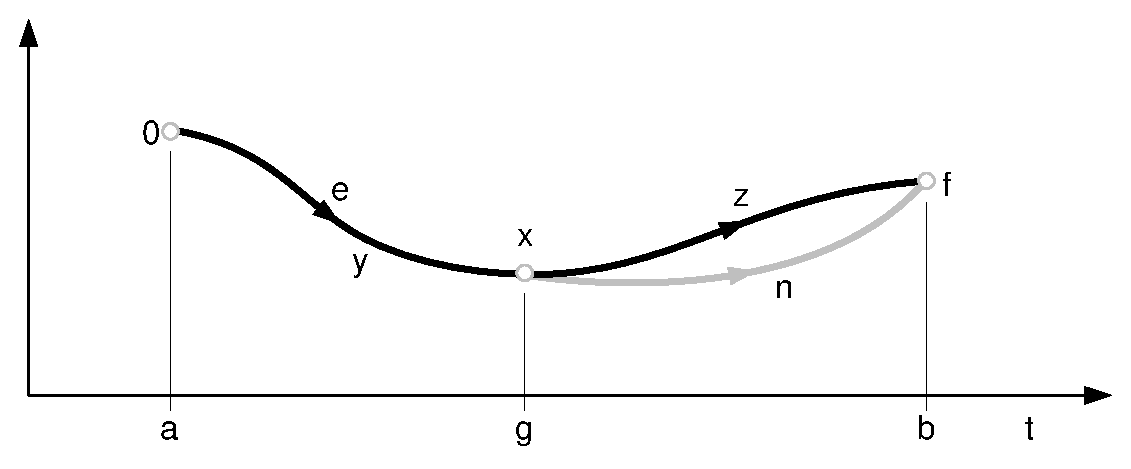
\includegraphics[width=1.0\textwidth,clip, trim = 0cm 0cm 0cm 0cm]{7_Darstellung_Bellmanprinzip.eps}
	\caption[Zur Verdeutlichung des Bellman'schen Optimalitätsprinzips]{Zur Verdeutlichung des Bellman'schen Optimalitätsprinzips \cite{foellingeroptimal}} 
	\label{fig:Darstellung_Bellmanprinzip}
\end{figure} 

Das Optimalitätsprinzip mag zwar intuitiv naheliegend sein, es führt aber zu einer ganzen Reihe von Optimierungsverfahren, die unter den Begriff der \emph{Dynamischen Programmierung} fallen und auf der \emph{Bellman'schen Rekursionsformel}\index{Bellman'schen Rekursionsformel} basieren. Letztere wird nachfolgend hergeleitet (s.\ \zB \cite{foellingeroptimal, papageorgiou2012optimierung}).



Die Bellman'sche Behandlung von \emph{zeitkontinuierlichen} Optimierungsaufgaben stellt vor allem eine theoretische Ergänzung zum Maximumprinzip in Kap.\,\ref{chap:dynamische_Optimierung_indirekt} dar und führt auf die sog.\ \emph{Hamilton-Jacobi-Bellman-Gleichung}. Sie ist eine nichtlineare partielle Differentialgleichung 1.\,Ordnung, weshalb sich ihre praktische Anwendbarkeit auf einfache Problemstellungen beschränkt, s.\ \zB \cite{Sundar1997}. 
Die praktische Stärke des Optimalitätsprinzips liegt hingegen in der Lösung \emph{zeitdiskreter} Problemstellungen. \\
Aus dem Grund sei ein zeitdiskreter, zeitvarianter Prozess
\begin{align} \label{equ:diskreter_prozess}
	\bs x(k+1) = \bs f(\bs x(k), \bs u(k), k), \quad k=0,\ldots, k_f-1
\end{align}
betrachtet, für den die Steuerfolge $\bs u^\ast(k)$ gesucht wird, die zur Minimierung des Kostenfunktionals
\begin{align}
	J = \sum_{k=0}^{k_f-1} l(\bs x(k), \bs u(k),k) \label{equ:diskrete_kosten} %+ V(\bs x(k_f)) 
\end{align}
führt. Neben der Anfangsbedingung $\bs x(0) = \bs x_0 $ seien vereinfachend nur Endbedingungen  $\bs x(k_f) = \bs x_f$ betrachtet. Die Ergebnisse können jedoch auf Probleme mit freier Endzeit $k_f$ und Endbedingung $\bs g(\bs x(k_f))\!=\! \bs 0$ sowie Zustands- und Stellgrößenbeschränkungen\footnote{Bei der dynamischen Programmierung bietet sich häufig an, Verletzungen der Nebenbedingungen in Form von unendlich hohen Kosten in \eqref{equ:diskrete_kosten} zu bestrafen \cite{lavalle2006pa}.} unterschiedlicher Art übertragen werden.

Um das Optimalitätsprinzips anzuwenden, werden die sog.\ \emph{Überführungskosten}\index{Überführungskosten} (\emph{cost-to-go}) als
\begin{align*}
	G = \sum_{\kappa = k}^{k_f-1} l(\bs x(\kappa), \bs u(\kappa),\kappa) % + V(\bs x(k_f))
\end{align*}
definiert, welche von einem Zwischenzustand $\bs x(k)$ zum Erreichen des Endzustands anfallen. Die minimalen Überführungskosten $G^\ast$ hängen lediglich vom Anfangszustand $\bs x(k)$ und der Zeit $k$ ab, 
\begin{align} \label{equ:cost_to_go}
	G^\ast(\bs x(k),k) = \min_{\bs u(\kappa)} G = \min_{\bs u(\kappa)} \sum_{\kappa = k}^{k_f-1} l(\bs x(\kappa), \bs u(\kappa),\kappa) \;,
\end{align}
wobei über die \emph{gesamte} Steuerfolge $\bs u(\kappa)$ mit $\kappa = k, \ldots , k_f-1$ zu optimieren ist.
Durch Aufteilung der Überführungstrajektorie $\bs x(\kappa)$ an der Stelle $k+1$ und Anwendung des Optimalitätsprinzips wird
\begin{align*}
 G^\ast(\bs x(k),k) = \min_{\bs u(k)}\{\,l(\bs x(k), \bs u(k), k) + G^\ast(\bs x(k+1),k+1)\,\}
\end{align*}
erhalten. Einsetzen der Dynamik \eqref{equ:diskreter_prozess} führt schließlich auf die Gleichung
\begin{align*}
 G^\ast(\bs x(k),k) = \min_{\bs u(k)}\{\,l(\bs x(k), \bs u(k), k) + G^\ast(\bs f(\bs x(k), \bs u(k), k), k+1)\,\} \, ,
\end{align*}
die auch als \emph{Bellman'sche Rekursionsformel} bezeichnet wird. Im Unterschied zu \eqref{equ:cost_to_go} erfolgt hierin die Minimierung nur noch über die Steuergröße des $k$-ten Zeitpunktes, also $\bs u(k)$. Durch die Rekursion kann somit der ursprünglich mehrstufige Optimierungsprozess in $k_f$ einstufige Entscheidungsprobleme zerlegt werden. Nachfolgend wird erläutert, wie sich den Sachverhalt verschiedene Verfahren der dynamischen Programmierung zunutze machen.

\section{Suchalgorithmen}
\subsection{Wert-Iteration-Verfahren}\index{Wert-Iteration} \label{sec:wertiteratrion}
Vereinfachend sei zunächst angenommen, dass die Stellgröße $\bs u(k) \in \mathcal U(\bs x(k),k)$ nur diskrete Werte annehmen darf und dabei das System immer von einem diskreten Zustand $\bs x(k) \in \mathcal X(k)$ in einen der nachfolgenden diskreten Zustände überführt. Insgesamt entsteht dadurch ein $k_f$-stufiger Entscheidungsprozess\index{Entscheidungsprozess}, der in Abb.\,\ref{fig:dynamische_programmierung_veranschaulichung} als einfacher Fall mit skalarer Stellgröße $u$ und skalarem Zustand $x$ mit jeweils drei Diskretisierungswerten pro Zeitschritt %mit zeitvarianten Kosten $l(x(k), u(k), k)$
dargestellt ist.
% Erst naives Herangehen
% Föllinger
\begin{figure}[ht]
	\psfrag{0}[tc][tc][1.0]{0}
	\psfrag{1}[tc][tc][1.0]{1}
	\psfrag{2}[tc][tc][1.0]{2}
	\psfrag{3}[tc][tc][1.0]{3}
	\psfrag{4}[tc][tc][1.0]{$k_f$}
	\psfrag{5}[tc][tc][1.0]{$x(0) = x_0$}
	\psfrag{6}[bc][bc][1.0]{$x(k_f) = x_f$}
	\psfrag{t}[bc][bc][1.0]{$k$}
	\psfrag{o}[bl][bl][1.0]{$x^\ast(k)$}
	\psfrag{x}[bl][bl][1.0]{$x$}
	\psfrag{u}[tr][tr][1.0]{$u^\ast(0)$}
	\psfrag{g}[b][b][1.0]{$8$}
	\psfrag{a}[b][b][1.0]{$6$}
	\psfrag{b}[b][b][1.0]{$5$}
	\psfrag{c}[b][b][1.0]{$8$}
	\psfrag{s}[b][b][1.0]{$10$}
	\psfrag{v}[b][b][1.0]{$9$}
	\psfrag{d}[b][b][.7]{$2$}
	\psfrag{e}[b][b][.7]{$4$}
	\psfrag{f}[b][b][.7]{$1$}
	\psfrag{h}[b][b][.7]{$6$}
	\psfrag{i}[b][b][.7]{$5$}
	\psfrag{j}[b][b][.7]{$8$}
	\psfrag{m}[tr][tr][1.0]{$\min$}
	\psfrag{k}[b][b][.7]{$3$}
	\psfrag{l}[b][b][.7]{$5$}
	\psfrag{n}[b][b][.7]{$6$}
	\psfrag{p}[br][br][.7]{$1$}
	\psfrag{q}[br][br][.7]{$4$}
	\psfrag{r}[b][b][.7]{$3$}
	\psfrag{z}[b][b][1.0]{$11$}
	\psfrag{y}[tr][tr][1.0]{$\argmin{}$}
	\centering
  	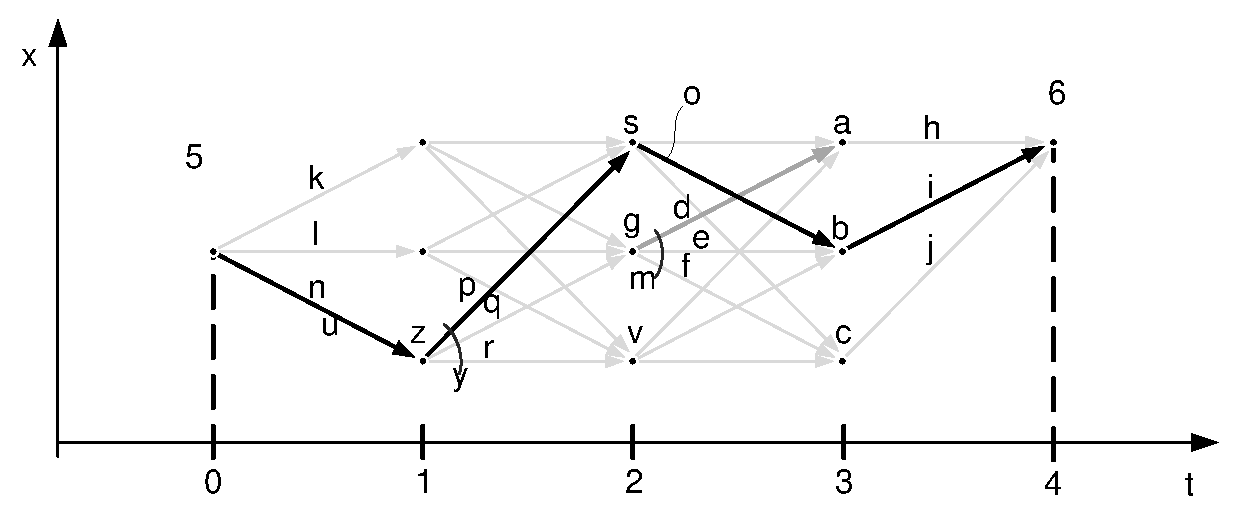
\includegraphics[width=0.98\textwidth,clip, trim = 0cm 0cm 0cm 0cm]{7_dynamische_programmierung_veranschaulichung.eps}
	\caption[Anwendungsbeispiel der Dynamischen Programmierung]{Anwendung der Dynamischen Programmierung auf ein kombinatorisches Problem, vgl.\ \cite{foellingeroptimal}}
	\label{fig:dynamische_programmierung_veranschaulichung}
\end{figure} 
Auch wenn hier der naive Lösungsweg über das Durchprobieren aller $3^3 = 27$ Möglichkeiten gangbar ist, so verbietet sich in jedem Fall diese Herangehensweise bei praktischen Problemstellungen mit einer höheren Stellgrößenanzahl $m$ und längeren Zeithorizonten $k_f$ aufgrund einer Laufzeit von  $\mathcal O(m^{k_f})$.

Zur Anwendung der Bellman'schen Rekursionsformel wird mit der letzten Stufe $k = k_f-1$ begonnen, für die zu jedem möglichen Zustand $\bs x(k) \in \mathcal X(k)$ die optimalen Überführungskosten $G^\ast(\bs x(k),k)$ berechnet und gespeichert werden. Beim in Abb.\,\ref{fig:dynamische_programmierung_veranschaulichung} betrachteten Beispiel erfordert das mit $k=3$ für jeden der drei Zustandswerte von $x(k)$ lediglich die Evaluation von $l(x(k), u(k), k)$ für das jeweils zum $x_f$ führende $u(k)$. \\
Im nächsten Schritt $k$ und in jedem darauffolgenden werden für alle $\bs x(k) \in \mathcal X(k)$ mit Hilfe der Rekursionsformel die optimalen Überführungskosten berechnet und abgelegt, getreu dem Motto: \emph{Falls der Zustand später Teil der optimalen Trajektorie ist, wie hoch sind hier die optimalen Kosten bis zum Ziel?} Dafür reicht es aus, für jedes zulässige $\bs u(k)$ die Kosten $l(\bs x(k), \bs u(k), k)$ zu evaluieren, diese zu den bereits für die nachfolgende Stufe berechneten Überführungskosten $G^\ast(\bs f(\bs x(k), \bs u(k),k),k+1)$ zu addieren und darüber das Minimum zu bestimmen, was bei $m$ Stellgrößen und $n$ Zuständen in $\mathcal O(m n)$ erfolgt. \\
Zuletzt wird $k=0$ erreicht, wo nur noch für den Anfangszustand $\bs x_0$ die Rekursionsformel ausgewertet werden muss, was die optimale Stellgröße $\bs u^\ast(0)$ liefert. Insgesamt führt somit dieses als \emph{Wert-Iteration} (\emph{value iteration}) bezeichnete Verfahren zu  einer Laufzeit von $\mathcal O(m n k_f)$. Es ist in Alg.\,\ref{alg:valueiteration} zusammengefasst.

Für eine optimale Regelung ist damit die Optimierung abgeschlossen, da $\bs u^\ast(0)$ gestellt und entsprechend des aktualisierten Anfangszustands von Neuem begonnen werden kann. Wird wie in den meisten praktischen Anwendungen die optimale Trajektorie $\bs x^\ast(k)$ gesucht, kann in jeder Stufe zu den optimalen Überführungskosten auch die zu diesen führende Stellgröße gespeichert werden. Alternativ ist die Trajektorie durch abwechselnde Auswertung von 
\begin{align} \label{equ:navigation_function}
\bs u^\ast(k) = \argmin{\bs u(k)}\{\,l(\bs x(k), \bs u(k), k) + G^\ast(\bs f(\bs x(k), \bs u(k),k), k+1)\,\}
\end{align}
und \eqref{equ:diskreter_prozess} zu berechnen, beginnend mit $\bs x_0$ hin zu $\bs x_f$, wobei die zuvor bestimmten Überführungskosten $G^\ast$ zu einer direkten Navigation zum Ziel verhelfen. Mehr noch: Da $G^\ast(\bs x, k)$ unabhängig vom Anfangszustand $\bs x_0$ berechnet wurde (das gilt im Übrigen auch bei der zuvor erwähnten Speicherung der Stellgröße), ist es durch die hier beschriebene \emph{rückwärtsgerichtete} Wert-Iteration möglich, für jeden beliebigen Zustand $\bs x$ von jeder Stufe $k$ aus die optimale Stell- und Zustandsfolge zu $\bs x_f$ zu bestimmen. Analog hierzu kann die Wert-Iteration \emph{vorwärtsgerichtet} durchgeführt werden, also mit den Zeitstufen von $k=0$ bis $k=k_f-1$, womit $\bs x_0$ optimal\footnote{Ein freier Endzustand erfordert typischerweise die Erweiterung von \eqref{equ:diskrete_kosten} um Endkosten $V(\bs x_f, k_f)$.} in jeden freien Zielzustand $\bs x_f \in \mathcal X(k_f)$ überführt werden kann. \\
%
%Auch wenn das Verfahren hier für diskrete Zustände dargestellt wurde (s.\ bspw.\ die Fahrzeuganwendung \cite{zieg09spatemp}), {\color{red} so stellt es vor allem eine effiziente Methode zur Berechnung optimaler Trajektorien im kontinuierlichen Zustandsraum dar \cite{lavalle2006pa}, die in Abschn.\,\ref{sec:dynamic_interpolation} genauer beleuchtet werden.} 
Der große Vorteil des stufenweisen Vorgehens der Wert-Iteration besteht darin, dass auf das teils recht aufwändige Mitführen einer Prioritätswarteschlange, wie sie für die im Anschluss dargestellten Verfahren vonnöten ist, verzichtet werden kann, s.\ beispielsweise die Trajektorienplanung \cite{zieg09spatemp}.

% ftp://ftp.tu-chemnitz.de/pub/tex/macros/latex/contrib/algorithms/algorithms.pdf

\renewcommand{\algorithmiccomment}[1]{// #1}
%%%\floatname{algorithm}{Algorithmus}
\begin{algorithm}[ht]
 \caption{Rückwärtsgerichtete Wert-Iteration \cite{papageorgiou2012optimierung}}
 \begin{algorithmic}[1]
	%\FORALL{$\bs x \in \mathcal X(k_f-1)$}
%\STATE $G(\bs x) \leftarrow \infty$
%\ENDFOR
	\STATE $G^\ast(\bs x_f,k_f) \leftarrow 0$
	\FOR {$k=k_f-1$ \TO $0$}
		\FORALL{$\bs x \in \mathcal X$}
			\STATE $G^\ast(\bs x(k),k) = \underset{\bs u(k)}{\min}\{\,l(\bs x(k), \bs u(k), k) + G^\ast(\bs f(\bs x(k), \bs u(k), k),k+1)\,\}$
		\ENDFOR
	\ENDFOR
 \end{algorithmic}
 \label{alg:valueiteration}
 \end{algorithm}

\subsection{Dijkstra-Suche\index{Dijkstra-Suche}}
Bei genauerer Betrachtung von Abb.\,\ref{fig:dynamische_programmierung_veranschaulichung} wird ersichtlich, dass die Systemdynamik eine Struktur beschreibt, die als \emph{Graph}\index{Graph} \cite{lavalle2006pa} interpretiert werden kann. Die sog.\ \emph{Knoten}\index{Knoten} (\emph{vertices}) repräsentieren hierin die diskreten Systemzustände $\bs x(k)$, verbunden über sog.\ \emph{Kanten}\index{Kante} (\emph{edges}), welche die durch $\bs u(k)$ herbeigeführten Zustandsübergänge zwischen ihnen darstellen. 
Genauer gesagt handelt es sich in Abb.\,\ref{fig:dynamische_programmierung_veranschaulichung} um einen \emph{gerichteten, azyklischen} Graphen, da zeitlich rückwärtsgerichtete Zustandsübergänge, die einen Zyklus entstehen lassen könnten, nicht möglich sind \cite{zieg09spatemp}. Erst hierdurch wird das stufenweise Vorgehen der zuvor vorgestellten Wert-Iteration durchführbar.

% http://en.wikipedia.org/wiki/Dijkstra's_algorithm
\renewcommand{\algorithmiccomment}[1]{// #1}
%%%\floatname{algorithm}{Algorithmus}
\begin{algorithm}[ht]
 \caption{Dijkstra-Suche \cite{lavalle2006pa}}
 \begin{algorithmic}[1]
\STATE $\mathcal Q = \emptyset$ 
\FORALL{$\bs x \in \mathcal X$}
\STATE $C(\bs x) \leftarrow \infty$ 				 \label{ln:dij:infty}
\STATE $\mathcal Q$.Insert($\bs x,C(\bs x)$) \label{ln:dij:q_insert}
\ENDFOR
\STATE $\bs x_0.\text{Predecessor} \leftarrow \text{null}$
\STATE $C(\bs x_0) \leftarrow 0$ 						 \label{ln:dij:zero}
\STATE $\mathcal Q$.DecreaseKey$(\bs x_0, C(\bs x_0))$ \label{ln:dij:q_decrease1}
\WHILE{$\mathcal Q\neq \emptyset$}
	\STATE $\bs x \leftarrow \mathcal Q$.ExtractMin$()$ \label{ln:dij:ExtractMin}
	\IF {$\bs x = \bs x_f$}
		\STATE \textbf{return} SolutionFound \label{ln:dij:xf}
	\ELSE 
		\FORALL{$\bs u \in \mathcal U(\bs x)$}
			\STATE $\tilde{\bs x} \leftarrow \bs f(\bs x,\bs u)$ \label{ln:dij:x_next}
			\STATE $\tilde C \leftarrow C(\bs x) + l(\bs x, \bs u)$
			\IF{ $ \tilde C < C(\tilde{\bs x}) $}
			\STATE $\tilde{\bs x}.\text{Predecessor}=\bs x$ \label{ln:dij:predesessor}
			\STATE $C(\tilde{\bs x}) \leftarrow \tilde C$
			\STATE $\mathcal Q$.DecreaseKey$(\tilde{\bs x},C(\tilde{\bs x}))$ \label{ln:dij:q_decrease}
			\ENDIF
		\ENDFOR
	\ENDIF
\ENDWHILE
\STATE \textbf{return} SolutionNotFound \label{ln:dij:nosolution}
 \end{algorithmic}
 \label{alg:Dijkstra}
 \end{algorithm}

Inmitten eines statischen Fahrzeugumfelds wie parkende Autos ist das Optimierungsproblem \emph{zeitinvariant}, da dann neben dem Fahrzeugmodell auch das Kostenfunktional und die Nebenbedingungen nicht von der Zeit $k$ abhängen. Um den Suchgraphen klein zu halten, empfiehlt es sich dann, identische Zustände von unterschiedlichen Zeitpunkten durch denselben Knoten zu repräsentieren. Als Beispiel sei die optimale Routenwahl in einem Straßennetz genannt, bei der es \iA nicht darauf ankommt, zu welcher Zeit eine Kreuzung angefahren wird. \\
%in Abb.\,\ref{fig:dijkstra} dargestellt ist. \\
Da das Problem nunmehr keine Zeitabhängigkeit aufweist, %(und im Straßennetzbeispiel zusätzlich die Kanten ungerichtet sind) 
sind Zyklen möglich, sodass von einem \emph{zyklischen} Graphen gesprochen wird. Für die Optimierung erweist sich dann aber das Fehlen einer für die Wert-Iteration erforderlichen topologischen Ordnung (über $k$) als nachteilig. Um dennoch das Prinzip der dynamischen Programmierung systematisch anwenden zu können, tritt an ihre Stelle beim \emph{Dijkstra}-Algorithmus eine sog.\ \emph{Prioritätswarteschlange} (\emph{queue}), deren Aufgabe nun erläutert wird. \\ %Zuvor sind jedoch noch die \emph{akkumulierten Kosten} (\emph{cost-to-come}) mit 
%\begin{align}
	%C(\bs x) = \sum_{\kappa=0}^{k}l(\bs x(\kappa), \bs u(\kappa))
%\end{align}
Mit $\mathcal Q$ wird eine Warteschlange bezeichnet, deren Elemente Knoten des Suchgraphen sind, und welche die  Reihenfolge bei der Anwendung der Rekursionsformel dynamisch festlegt.  Sie wird entsprechend einer Funktion $C: \mathcal X \rightarrow [0,\infty]$ sortiert, welche als \emph{akkumulierte Kosten} (\emph{cost-to-come}) bezeichnet wird. Analog zu $G^\ast$ werden die minimalen akkumulierten Kosten $C^\ast(\bs x)$ erhalten, wenn alle Verbindungen (sog.\ \emph{Pfade}) herangezogen werden, die den Anfangszustand $\bs x_0$ in $\bs x$ überführen, und die akkumulierten Kosten zu dem Pfad ausgewählt werden, der zu der geringsten Summe über $l(\bs x, \bs u)$ führt. Hierbei wird angenommen, dass für alle Kanten $l(\bs x, \bs u)>0$ gilt. Ganz vorne in $\mathcal Q$ steht also immer das Element $\bs x$ mit den geringsten akkumulierten Kosten $C^\ast(\bs x)$.
%
%
\begin{figure}[ht]
\newcommand{\smallsize}{.75}
	\psfrag{M}[cl][cl][1.0]{M}
	\psfrag{S}[tr][tr][1.0]{S}
	\psfrag{L}[cl][cl][1.0]{L}
	\psfrag{F}[cr][cr][1.0]{F}
	\psfrag{h}[bc][bc][1.0]{H}
	\psfrag{q}[cl][cl][\smallsize]{$C\!=\!0$}
	\psfrag{s}[cr][cr][\smallsize]{$C\!=\!230$}
	\psfrag{l}[tl][tl][\smallsize]{$C\!=\!424$}
	\psfrag{f}[cr][cr][\smallsize]{$C\!=\!454$}
  \psfrag{x}[bl][bl][\smallsize]{$C\!=\!684$}
  \psfrag{1}[tr][tr][\smallsize]{$230$}
	\psfrag{2}[tl][tl][\smallsize]{$424$}
  \psfrag{3}[br][br][\smallsize]{$470$}
  \psfrag{4}[tr][tr][\smallsize]{$224$}
  \psfrag{5}[br][br][\smallsize]{$350$}
  \psfrag{6}[bl][bl][\smallsize]{$260$}
 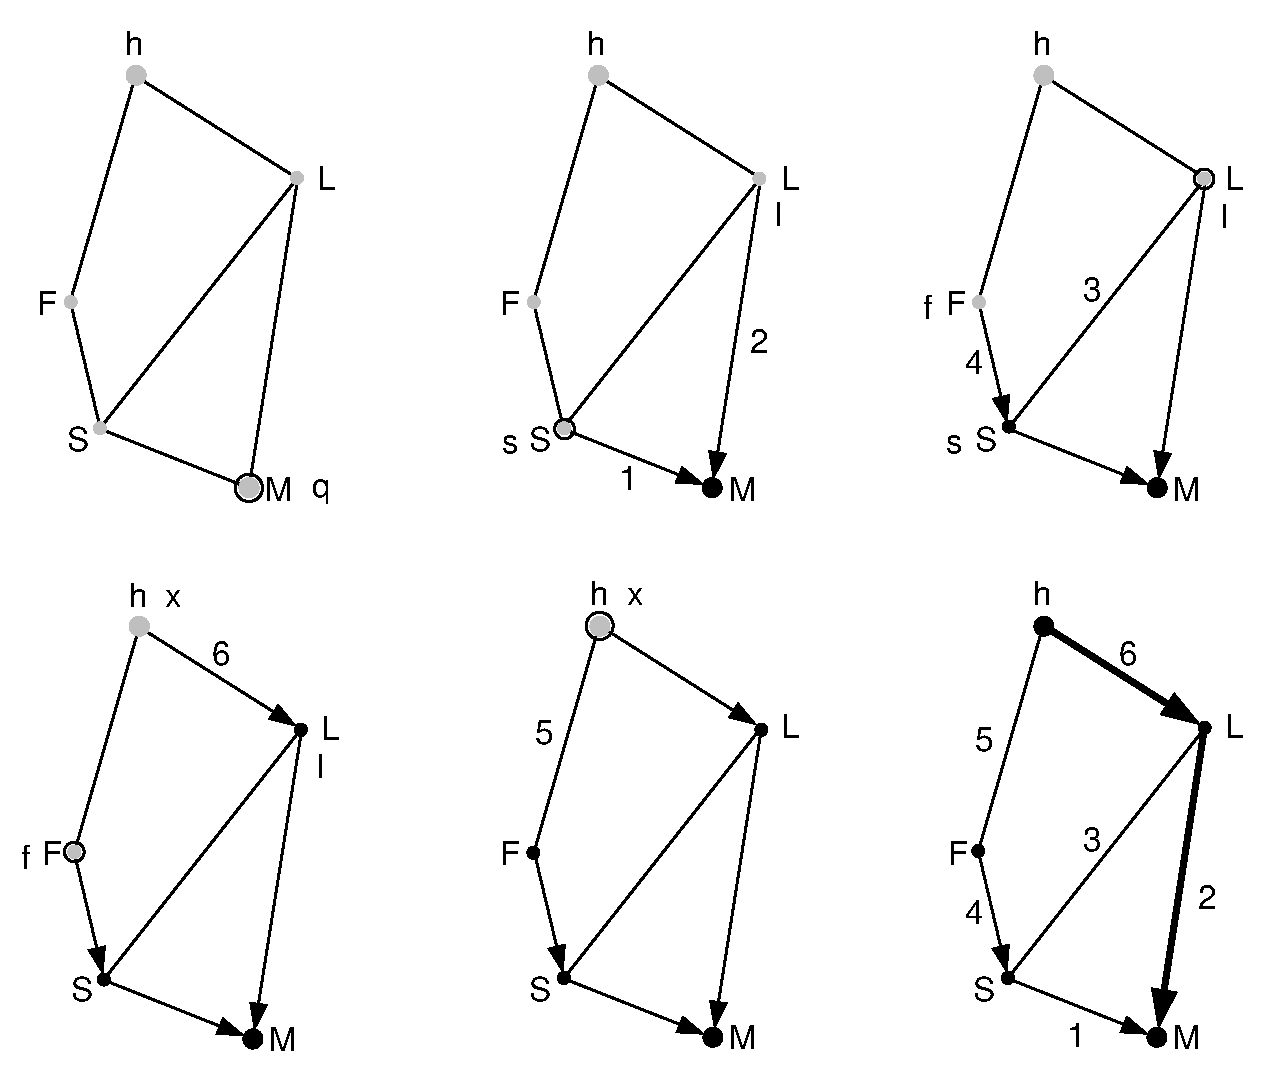
\includegraphics[width=.9\textwidth,clip, trim = 0cm 0cm 0cm 0cm]{7_Dijkstra.eps}
	\caption[Dijkstra-Suche zur Bestimmung des kürzesten Wegs]{Dijkstra-Suche zur Bestimmung der kürzesten Verbindung zwischen Startknoten M und Zielknoten H eines Straßennetzes; der schwarze Kreis markiert den im jeweiligen Schritt (beginnend oben links) expandierten Knoten; schwarz sind alle Knoten, die von der Prioritätswarteschlange entfernt und damit bereits expandiert wurden.} 
	\label{fig:dijkstra}
\end{figure}

Wie schon bei $G^\ast(\bs x(k), k)$ der Wert-Iteration erfolgt auch bei der Dijkstra-Suche die Berechnung von $C(\bs x)$ inkrementell, s.\ Alg.\,\ref{alg:Dijkstra}. %bzw.\  $C^\ast(\bs x)$
Zunächst werden die akkumulierten Kosten aller Knoten mit $\infty$ initialisiert und der Prioritätswarteschlange $\mathcal Q$ hinzugefügt (Zeilen~\ref{ln:dij:infty}, \ref{ln:dij:q_insert}). $C(\bs x_0)$ wird anschließend auf $0$ gesetzt und in $\mathcal Q$ aktualisiert (Z.\,\ref{ln:dij:zero}, \ref{ln:dij:q_decrease1}), womit der Startknoten ganz nach vorne wandert. \\
Solange sich nun noch Elemente in $\mathcal Q$ befinden, wird immer das Element $\bs x$ mit dem geringsten $C$-Wert\footnote{Für dieses Element $\bs x$ sind demnach die minimalen akkumulierten Kosten bekannt, sodass es sich tatsächlich um $C^\ast(\bs x)$ handelt.} entfernt (Z.\,\ref{ln:dij:ExtractMin}). Stellt es den Zielknoten $\bs x_f$ dar, so ist die Suche beendet (Z.\,\ref{ln:dij:xf}). Andernfalls wird der Knoten $\bs x$ \emph{expandiert}, d.h. jeder Nachfolgeknoten $\tilde{\bs x}$ berechnet (Z.\,\ref{ln:dij:x_next}), und die Kosten $\tilde C = C(\bs x) + l(\bs x, \bs u)$ bestimmt, wobei $l(\bs x, \bs u)$ die Kosten von $\bs x$ nach $\tilde{\bs x}$ bezeichnen. Fällt $\tilde C$ geringer aus als $C(\tilde{\bs x})$, so wurde eine bessere Lösung nach $\tilde{\bs x}$ gefunden als zuvor berechnet, sodass durch $C(\tilde{\bs x})\leftarrow \tilde C$ die geringeren Kosten gespeichert werden, der Vorgängerknoten zu merken ist
 (Z.\,\ref{ln:dij:predesessor}) und $\tilde{\bs x}$ weiter vorne in $\mathcal Q$ einsortiert werden muss  (Z.\,\ref{ln:dij:q_decrease}). Hat sich $\mathcal Q$ komplett geleert, so gibt es keine Verbindung zwischen $\bs x_0$ und $\bs x_f$ und damit keine Lösung zum Problem (Z.\,\ref{ln:dij:nosolution}). Insgesamt ergibt sich bei $n$ Knoten, $m$ Kanten und einer geeigneten Datenstruktur für $\mathcal Q$ eine Laufzeit von $\mathcal O(n \log n + m)$ \cite{lavalle2006pa}. 
Der optimale Pfad lässt sich schließlich leicht mittels Iteration über die abgespeicherten Vorgänger (Z.\,\ref{ln:dij:predesessor}) ermitteln.

Anhand von Abb.\,\ref{fig:dijkstra} kann die Dijkstra-Suche nach der optimalen (kürzesten) Verbindung innerhalb eines Straßennetzes nachvollzogen werden.



% unterschiedliche Längen Pfadplanung in unstrukt. umgebung
% aber auch bei endzeit frei
\subsection{A$^\ast$-Suche\index{A$^\ast$-Suche}} \label{sec:astern}
Die A$^\ast$-Suche\footnote{ausgesprochen \emph{A Stern Suche}} stellt eine Erweiterung der Dijkstra-Suche dar, die möglichst wenige Knoten expandiert, indem sie \emph{zielgerichtet} vorgeht. 
Hierzu benötigt der Algorithmus eine Schätzfunktion $\hat {G}^\ast$ der minimalen Kosten bis zum Ziel, die sog.\ \emph{Heuristik}\index{Heuristik}. Um eine intuitive Vorstellung dieser Erweiterung zu vermitteln, sei erneut das Beispiel aus Abb.\,\ref{fig:dijkstra} betrachtet. Zur Motivation des Algorithmus wird jedoch jetzt angenommen, dass sich das der Suche zugrundeliegende Straßennetz vom Knoten M aus nicht nur nach Nord-Westen, sondern in alle anderen Himmelsrichtungen erstreckt. Da sich die Dijkstra-Suche bei der Expansion in jedem Schritt auf denjenigen Knoten konzentriert, der die geringsten akkumulierten Kosten $C$ vom Startpunkt aufweist, werden die Knoten dann in alle Himmelsrichtungen expandiert, sodass der Zielknoten H erst nach vielen Schritten erreicht wird. \\
Die Vorgehensweise beim A$^\ast$ unterscheidet sich nun von der Dijkstra-Suche dahingehend, dass nunmehr immer der Knoten expandiert wird, der die \emph{geringsten Gesamtkosten} $\hat J(\bs x)  = C(\bs x) + \hat {G}^\ast(\bs x)$ \emph{verspricht}, womit sich die "`Expansionsfront"' tendenziell in Richtung Zielknoten ausbreitet. Als Heuristik $\hat {G}^\ast(\bs x)$ bietet sich im Beispiel die "`Luftlinie"', also der euklidische Abstand, zur Zielstadt an, da sie einfach berechnet werden kann und die tatsächlich noch zurückzulegende Strecke \emph{optimistisch}
einschätzt. \\ 
Grundsätzlich ist nämlich eine Heuristik $\hat {G}^\ast(\bs x)$ \emph{zulässig}, wenn sie die Kosten bis zum Ziel \emph{nicht überschätzt}. In aller Regel kommen \emph{monotone} (auch \emph{konsistente})  Heuristiken zum Einsatz, d.h. solche, die nicht nur zulässig sind sondern auch noch die Dreiecksungleichung erfüllen.\footnote{Die geschätzten Kosten direkt zum Ziel dürfen höchstens so groß sein, wie die geschätzten Kosten eines beliebigen benachbarten Knoten zum Ziel zzgl.\ der tatsächlichen Übergangskosten zum Nachbarknoten. Ist die Heuristik nur zulässig, nicht aber monoton, dann ist zu einem expandierten Knoten nicht unbedingt der kürzeste Weg bekannt. Damit darf keine geschlossene Liste $\mathcal C$, s.\ Alg.\,\ref{alg:AStar}, eingesetzt werden, da es möglich sein muss, den Knoten mehrfach zu expandieren.} Eine gute Heuristik $\hat {G}^\ast$ zeichnet sich generell dadurch aus, dass sie die wahren Kosten $G^\ast$ so wenig wie möglich unterschätzt (da dann nur wenige Knoten expandiert werden müssen) und schnell zu bestimmen ist. Für die triviale Heuristik $\hat {G}^\ast = 0$ degeneriert die A$^\ast$-Suche zur Dijkstra-Suche.
 Grundsätzlich ist für eine zulässige Heuristik garantiert, dass die A$^\ast$-Suche immer die optimale Lösung findet \cite{lavalle2006pa}. \\
%
Da beim Einsatz einer guten Heuristik nur ein kleiner Teil der Knoten des Graphen expandiert wird, bietet es sich an, ihn erst zur Programmlaufzeit dynamisch aufzubauen (\emph{impliziter Graph}\footnote{Knoten und Kanten liegen nicht im Speicher, sondern werden erst zur Laufzeit bestimmt.}), womit gegenüber Alg.\,\ref{alg:Dijkstra} die Initialisierung aller Knoten mit $\infty$ und ihr Hinzufügen zur Warteschlange $\mathcal Q$ entfällt. Die Aufgabe von $\mathcal Q$  übernimmt jetzt die Prioritätswarteschlange $\mathcal O$, welche auch als \emph{offene Liste} (\emph{open list}) bezeichnet wird. Sollen Knoten nicht mehrfach untersucht werden, so wird mit einer \emph{geschlossenen Liste} $\mathcal C$ (\emph{closed list}) gearbeitet, die all jene Knoten beinhaltet, zu denen der optimale Pfad mit $C^\ast(\bs x)$ bekannt ist.

% http://de.wikipedia.org/wiki/A*-Algorithmus
\renewcommand{\algorithmiccomment}[1]{// #1}
\begin{algorithm}[!ht]
 \caption{A*-Suche \cite{lavalle2006pa}}
 \begin{algorithmic}[1]
\STATE $\mathcal O = \emptyset$ 
\STATE $\mathcal C = \emptyset$
\STATE $\bs x_0.\text{Predecessor} \leftarrow \text{null}$
\STATE $\hat J \leftarrow \hat G(\bs x_0)$
\STATE $\mathcal O$.Insert($\bs x_0, \hat J $) \label{ln:A:insert1}
\WHILE{$\mathcal O\neq \emptyset$}
	\STATE $\bs x \leftarrow \mathcal O$.ExtractMin() \label{ln:A:ExtractMin}
	\STATE $\mathcal C$.Insert($\bs x$) \label{ln:A:addcl}
	\IF {$\bs x = \bs x_f$}
		\STATE \textbf{return} SolutionFound \label{ln:A:solutionfound}
	\ELSE 
		\FORALL{$\bs u \in \mathcal U(\bs x)$} 
			\STATE $\tilde{\bs x} \leftarrow \bs f(\bs x,\bs u)$ \label{ln:A:exp}
			\IF{$\tilde{\bs x} \notin \mathcal C$}
				\STATE $\tilde C \leftarrow C(\bs x) + l(\bs x, \bs u)$
				\IF{$\tilde{\bs x} \notin \mathcal O$ \OR $\tilde C < C(\tilde{\bs x})$}
					\STATE $\tilde{\bs x}.\text{Predecessor}\leftarrow \bs x$ \label{ln:A:predesessor}
					\STATE $C(\tilde{\bs x}) \leftarrow \tilde C$
					\STATE $\hat J  \leftarrow C(\tilde{\bs x}) + \hat {G}^\ast(\tilde{\bs x})$
					\IF{$\tilde{\bs x} \notin \mathcal O$}
						\STATE $\mathcal O$.Insert($\tilde{\bs x},\hat J $) \label{ln:A:insert2}
					\ELSE
						\STATE $\mathcal O$.DecreaseKey($\tilde{\bs x},\hat J $) \label{ln:A:decrease}
					\ENDIF
				\ENDIF
			\ENDIF
		\ENDFOR
	\ENDIF
\ENDWHILE
\STATE \textbf{return} SolutionNotFound \label{ln:A:nosolution}
\end{algorithmic}
\label{alg:AStar}
\end{algorithm}

Zunächst ist $\mathcal C$ leer und $\mathcal O$ umfasst nur den Startknoten $\bs x_0$ mit $\hat J  = \hat G$, s.\ Alg.\,\ref{alg:AStar} in Z.\,1-\ref{ln:A:insert1}. In jedem Schritt wird nun der aussichtsreichste Knoten expandiert, also das vorderste Element von $\mathcal O$  (Z.\,\ref{ln:A:ExtractMin}), was gleichzeitig den Graphen aufbaut. Damit ist der Knoten abschließend untersucht und er wird der geschlossenen Liste $\mathcal C$ hinzugefügt (Z.\,\ref{ln:A:addcl}). Ein jeder seiner Nachfolgeknoten  (Z.\,\ref{ln:A:exp}), der sich noch nicht auf $\mathcal C$ befindet, wird entsprechend seiner geschätzten Gesamtkosten $\hat J := C(\bs x) + \hat G(\bs x)$ in $\mathcal O$ einsortiert  (Z.\,\ref{ln:A:insert2}). Falls er sich jedoch dort schon befindet und der neue Pfad zu ihm geringere Kosten verursacht als der bisherige, wird er entsprechend $\hat J $ innerhalb von $\mathcal O$ höher priorisiert  (Z.\,\ref{ln:A:decrease}).  Der Algorithmus terminiert, falls der Zielknoten an die erste Stelle von $\mathcal O$ gewandert ist (Z.\,\ref{ln:A:solutionfound}), sodass die optimale Lösung gefunden wurde, oder sich die offene Liste $\mathcal O$ geleert hat, womit keine Lösung existiert  (Z.\,\ref{ln:A:nosolution}).

Zur Verdeutlichung des Vorgehens dient die in Abb.\,\ref{fig:astar}  dargestellte A$^\ast$-Suche innerhalb eines gegenüber Abb.\,\ref{fig:dijkstra} vergrößerten Straßennetzes. Es sei darauf hingewiesen, dass im Unterschied zur Dijkstra-Suche der Knoten F nicht expandiert wird, obwohl der Pfad zum Zielknoten HH sogar länger ist.

\begin{figure}[h]
\newcommand{\cost}[3]{\parbox[t]{1.5cm}{\flushright $#1$ \\$\underline{#2}$ \\ $\bs{#3}$}}
\centering
\newcommand{\smallsize}{.75}
	\psfrag{H}[cb][cb][1.0]{HH}
		\psfrag{k}[lc][lc][\smallsize]{\cost{C\!=\!834}{G\!=\;\;\;0}{834}}
	\psfrag{r}[lc][lc][\smallsize]{$C\!=\!834$}
	\psfrag{h}[rb][rb][1.0]{H}
		\psfrag{i}[rc][rc][\smallsize]{\cost{C\!=\!684}{G\!=\!130}{814}}
	\psfrag{o}[rb][rb][\smallsize]{$C\!=\!684$}
	\psfrag{S}[rt][rt][1.0]{S}
	\psfrag{s}[rc][rc][\smallsize]{\cost{C\!=\!230}{G\!=\!530}{760}}
	\psfrag{a}[rt][rt][\smallsize]{$C\!=\!230$}
	\psfrag{M}[lc][lc][1.0]{M}
	\psfrag{m}[lc][lc][\smallsize]{$C\!=\!0$}
	\psfrag{z}[lc][lc][\smallsize]{\cost{C\!=\;\;\;0}{G\!=\!612}{612}}
	\psfrag{q}[rc][rc][\smallsize]{$C\!=\!454$}
	\psfrag{B}[bl][bl][1.0]{B}
	\psfrag{b}[lc][lc][\smallsize]{\cost{C\!=\!614}{G\!=\!255}{869}}
	\psfrag{v}[bl][bl][\smallsize]{$C\!=\!614$}
	\psfrag{L}[cb][cb][1.0]{L}
	\psfrag{l}[lc][lc][\smallsize]{\cost{C\!=\!424}{G\!=\!295}{719}}
	\psfrag{c}[lt][lt][\smallsize]{$C\!=\!424$}
	\psfrag{F}[cr][cr][1.0]{F}
	\psfrag{f}[rc][rc][\smallsize]{\cost{C\!=\!454}{G\!=\!390}{844}}
	\psfrag{1}[tr][tr][\smallsize]{$230$}
	\psfrag{2}[tl][tl][\smallsize]{$424$}
	\psfrag{3}[br][br][\smallsize]{$470$}
	\psfrag{4}[tl][tl][\smallsize]{$224$}
	\psfrag{5}[br][br][\smallsize]{$350$}
	\psfrag{6}[bl][bl][\smallsize]{$260$}
	\psfrag{7}[tl][tl][\smallsize]{$190$}
	\psfrag{8}[bl][cl][\smallsize]{$290$}
	\psfrag{9}[cr][cr][\smallsize]{$150$}
	\psfrag{0}[cr][cr][\smallsize]{$285$}
	
 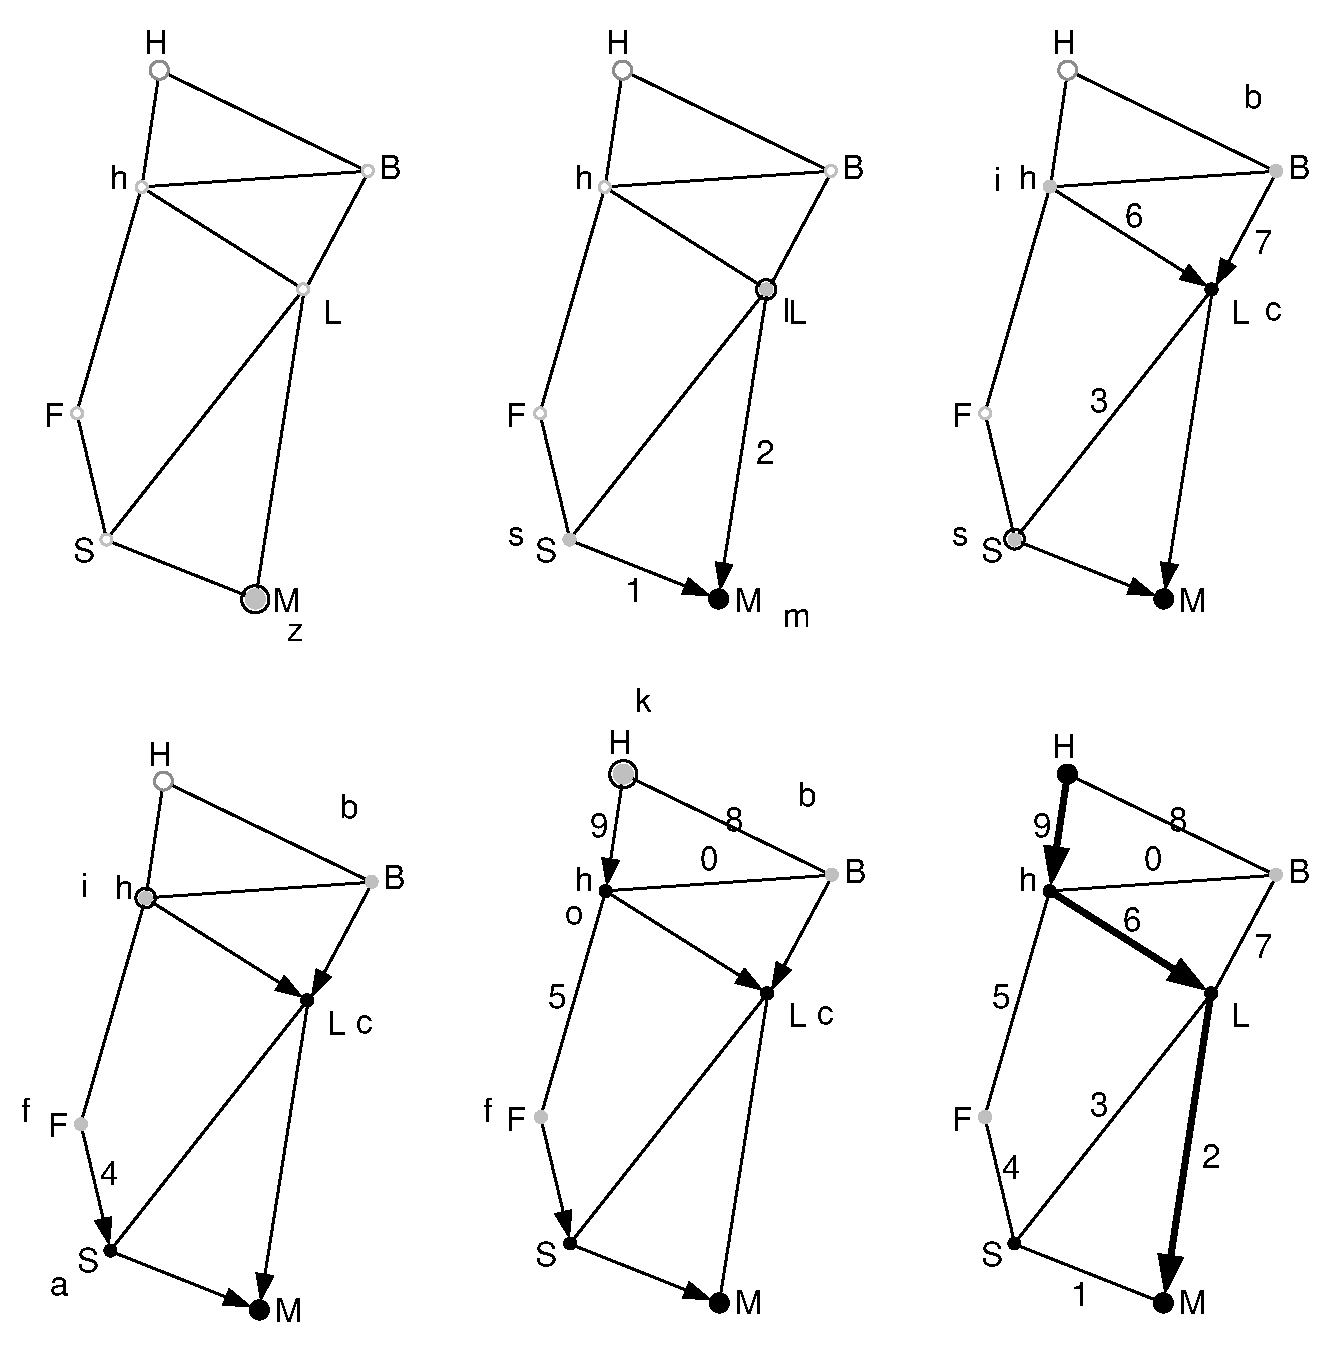
\includegraphics[width=.88\textwidth,clip, trim = 0cm 0cm 0cm 0cm]{7_A_star.eps}
	\caption[A*-Suche zur Bestimmung des kürzesten Wegs]{A*-Suche zur Bestimmung der kürzesten Verbindung zwischen Startknoten M und Zielknoten HH eines Straßennetzes; der schwarze Kreis markiert den im jeweiligen Schritt expandierten Knoten, der damit von der offenen Liste $\mathcal O$ (graue Knoten) auf die geschlossene Liste $\mathcal C$ (schwarze Knoten) wandert; Knoten, die noch nicht Teil des sich dynamisch aufbauenden Graphen sind, werden weiß dargestellt; $G := \hat {G}^\ast$}
	\label{fig:astar}
\end{figure} 

\section{Fahrzeugspezifische Problemformulierungen}
Da es sich bei der Optimalsteuerung zunächst um ein unendlich-dimensionales Problem handelt, s.\ Abschn.\,\ref{sec:unendlichdim_opt}, ist zur Anwendung der Dynamischen Programmierung %, wie schon bei den direkten Optimierungsmethoden in Kap.\,\ref{chap:dynamische_Optimierung_direkt}, 
eine Reduktion auf einen diskreten %, endlich-dimensionales Problem vonnöten, also auf einen 
Entscheidungsprozess vonnöten.
Im Kontext der Trajektorienoptimierung für Fahrzeuge ist häufig von sog.\ \emph{Bewegungsprimitiven}\index{Bewegungsprimitive} (\emph{motion primitives}) die Rede, aus denen die optimale Trajektorie zusammenzusetzen ist.
%Bei den in diesem Kapitel beschriebenen Optimierungsverfahren setzt sich die optimale Trajektorie aus sog.\ \emph{Bewegungsprimitiven} (\emph{motion primitives}) zusammen.
Hierbei
muss bei der Problemdiskretisierung zwischen den Gesichtspunkten \emph{Optimalität} (Wie stark weicht die Lösung des diskretisierten Problems vom ursprünglichen kontinuierlichen ab?), \emph{Vollständigkeit} (Beinhalten die Bewegungsprimitive alle für das Problem wesentlichen Trajektorien?) und \emph{Komplexität} (Wird durch die Diskretisierung das Problem für die Graphensuche hinreichend vereinfacht?) abgewogen werden \cite{lavalle2006pa, pivtoraiko2009differentially}. Im Folgenden werden zwei praxiserprobte Verfahren zur Generierung von Bewegungsprimitiven vorgestellt, die sich darin unterscheiden, dass im einen Fall die Diskretisierung (auch als \emph{Sampling} bezeichnet) über den Zustand  $\bs x$, im anderen Fall %, s.\ Absch.\,\ref{sec:lattice} 
über die Stellgröße $\bs u$ erfolgt.

\subsection{Inverse Bewegungsprimitive}
Um den Zustandsraum möglichst gleichmäßig abzudecken (es wird auch von minimaler \emph{Dispersion} gesprochen \cite{lavalle2006pa}), wird bei einem sog.\ \emph{Zustandsgitter}\index{Zustandsgitter} (\emph{state lattice}) \cite{pivtoraiko2007optimal} ein Sampling in einem Muster verfolgt. Seine kleinste, wiederkehrende Einheit wird als \emph{Steuermenge}\index{Steuermenge} (\emph{control set)} bezeichnet. 
Als anschauliches Beispiel zeigt hierzu Abb.\,\ref{fig:lattice} einen recht grob auflösenden Graphen mit einer Positionsdiskretisierung $\Delta x\!=\!\Delta y \!=\! \unit[10]{m}$ zu den nächsten drei Nachbarn, vier Endausrichtungen{ $\theta \in \{0, \nicefrac{1}{2}\,\pi, \pi, \nicefrac{3}{2}\,\pi \}$ und einer einzigen Endkrümmung  $\kappa = 0$. \\
%
\begin{figure}[h]
\centering
  	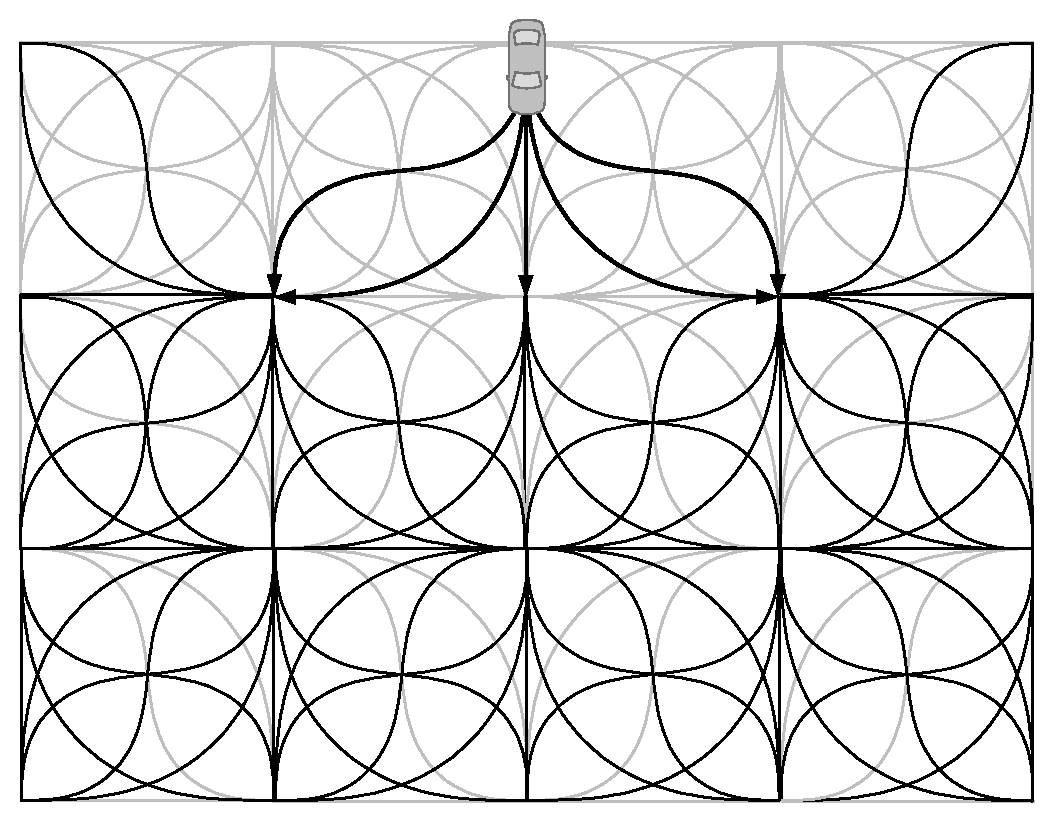
\includegraphics[width=.75\textwidth,clip, trim = 0cm 0cm 0cm 0cm]{7_Lattice.eps}
	\caption[Wiederkehrendes Sampling im Zustandsraum]{Wiederkehrendes Sampling im Zustandsraum führt zu einem Zustandsgitter, hier für die Vorwärtsfahrt in einer unstrukturierten Umgebung wie auf Parkplätzen; es werden alle in drei Expansionsschritten erreichbaren Zustände in Schwarz dargestellt; Darstellung basierend auf \cite{mcnaughton}}
	\label{fig:lattice}
\end{figure}

Generell muss bei der Berechnung der Steuermenge darauf geachtet werden, dass die Übergänge zwischen jedem diskreten Zustand $\bs x$ und seinen Nachbarzuständen nicht nur für das (vereinfachte) Fahrzeugmodell realisierbar, sondern auch vorteilhaft, wenn nicht gar optimal, im Sinne des Gütekriteriums sind. Für sog.\ flache  Systemmodelle \cite{fliess1995fad}, s.\ Abschn.\,\ref{sec:flachheitbasierte_para}, wie dem kinematischen Einspurmodell, besteht hierzu die Möglichkeit, mittels Polynomen hinreichender Ordnung den Verlauf des flachen Ausgangs (etwa die Hinterachsposition) vorzugeben und anschließend die daraus ableitbaren Zustands- und Stellgrößenverläufe auf Einhaltung ihrer Beschränkungen (\zB maximale Krümmung) zu überprüfen. \\
Die Generierung eines jeden Elements der Steuermenge stellt wiederum ein Optimalsteuerungsproblem (mit festem Endzustand und freier oder fester Endzeit bzw.\ zurückgelegter Wegstrecke) dar, zu dessen Lösung sich in erster Linie die noch in Kap.\,\ref{chap:dynamische_Optimierung_direkt} vorzustellenden Methoden anbieten \cite{howard2007optimal}. Sie können offline berechnet und abgespeichert werden, sodass es hierbei problemlos möglich ist, exakt die im Gütefunktional veranschlagten Bewegungskosten und sämtliche Zustands- und Stellgrößenbeschränkungen direkt zu berücksichtigen. \\
Überhaupt zeichnet sich die Zustandsgittermethode aufgrund ihrer Translationsinvarianz dadurch aus, dass während der Suche wiederkehrende Berechnungen vorab gelöst und im Speicher abgelegt werden können und sich somit der online-Rechenaufwand stark reduzieren lässt. Hierzu zählen vor allem die Bewegungskosten und Rechenoperationen der Hinderniskosten \cite{pivtoraiko2007optimal}. \\
Diese Eigenschaft geht jedoch bei strukturierten Umgebungen wie Straßen weitestgehend verloren, wenn zur Minimierung der sog.\ \emph{Diskrepanz} \cite{lavalle2006pa} das Zustandsgitter an die Referenz angepasst wird, s.\ Abb.\,\ref{fig:lattice_strasse}, da es dann aufgrund des variablen Straßenverlaufs zur Laufzeit aufgebaut werden muss \cite{zieg09spatemp, mcnaughton}.
\begin{figure}[h]
\centering
  	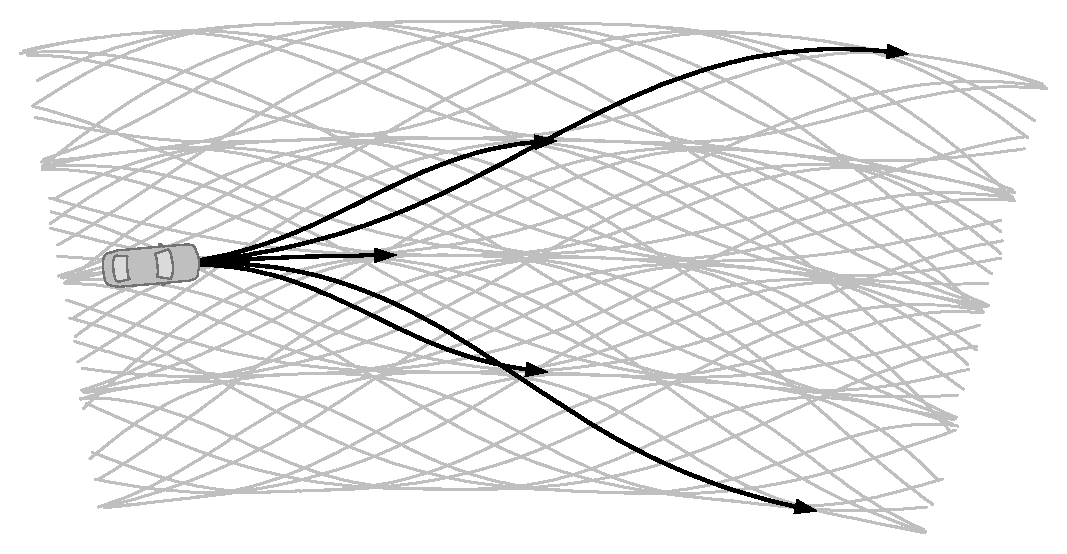
\includegraphics[width=.8\textwidth,clip, trim = 0cm 0cm 0cm 0cm]{7_Lattice_strasse.eps}
	\caption[Zustandsgitter für eine strukturierte Umgebung]{Zustandsgitter für eine strukturierte Umgebung wie Straßen; Steuermenge in Schwarz; Sollen dynamische Hindernisse berücksichtigt werden, muss die Zeit $t$ explizit berücksichtigt werden, sodass sich Wert-Iterationen zur Optimierung anbieten \cite{zieg09spatemp, mcnaughton}; Darstellung basierend auf \cite{McNaughton2011diss}}
	\label{fig:lattice_strasse}
\end{figure}

\subsection{Vorwärtssimulierte Bewegungsprimitive}
Als nachteilig erweist sich bei der zuvor dargestellten Herangehensweise, dass das exakte Erreichen von den diskreten Zuständen der Stellgröße einen teils sehr unnatürlichen Verlauf aufprägt. So fallen in Abb.\,\ref{fig:lattice} die erforderlichen Lenkbewegungen mit Verkleinerung von $\Delta x$, $\Delta y$ immer extremer aus. \\
Um das Problem zu umgehen, können die Bewegungsprimitive durch Vorwärtssimulation unterschiedlicher, abschnittsweise konstanter Stellgrößen berechnet werden \cite{zieglerIV08, dolgov2010path}, s.\ Abb.\,\ref{fig:pruning}. Die gegenüber dem Zustandsgitter verbesserten Stellgrößenverläufe werden jedoch damit erkauft, dass die Knoten des sich so errichtenden Suchgraphen \iA nicht übereinander liegen, sich also zunächst nur ein sog.\ Suchbaum ergibt. Um dessen exponentiellen Knotenwachstum entgegen zu wirken, welches die Suche über längere Horizonte klar verbietet, kann der Graph an den Knoten, deren Zustände sich nur unwesentlich voneinander unterscheiden, geschlossen\footnote{Die spezielle Graphenform des Baums geht dabei verloren. Der für das Graphenschließen häufig synonym verwendete Begriff \emph{pruning} (Stutzen) \cite{dolgov2010path} ist ein wenig irreführend, da hierbei nicht Äste abgeschnitten, sondern nur optimale Lösungen, ganz im Sinne der dynamischen Programmierung, weiterverfolgt werden.} werden. Implementierungstechnisch kann dieses auch als \emph{hybrid state} Suche \cite{dolgov2010path} bezeichnete Herangehen so umgesetzt werden, dass im Expansionsschritt der Graphensuche der Endzustand $\tilde{\bs x}$ auf eine bestimmte Auflösung  $\Delta \bs x$  gerundet wird und die offene (oder ggf.\ auch die geschlossene) Liste darauf überprüft wird, ob ein entsprechender Knoten schon existiert. Um dennoch stetig in den Zuständen zu sein, wird die Expansion immer von dem entsprechenden ungerundeten Endzustand fortgeführt \cite{dolgov2010path}. \\ 

\begin{figure}[h]
\centering
 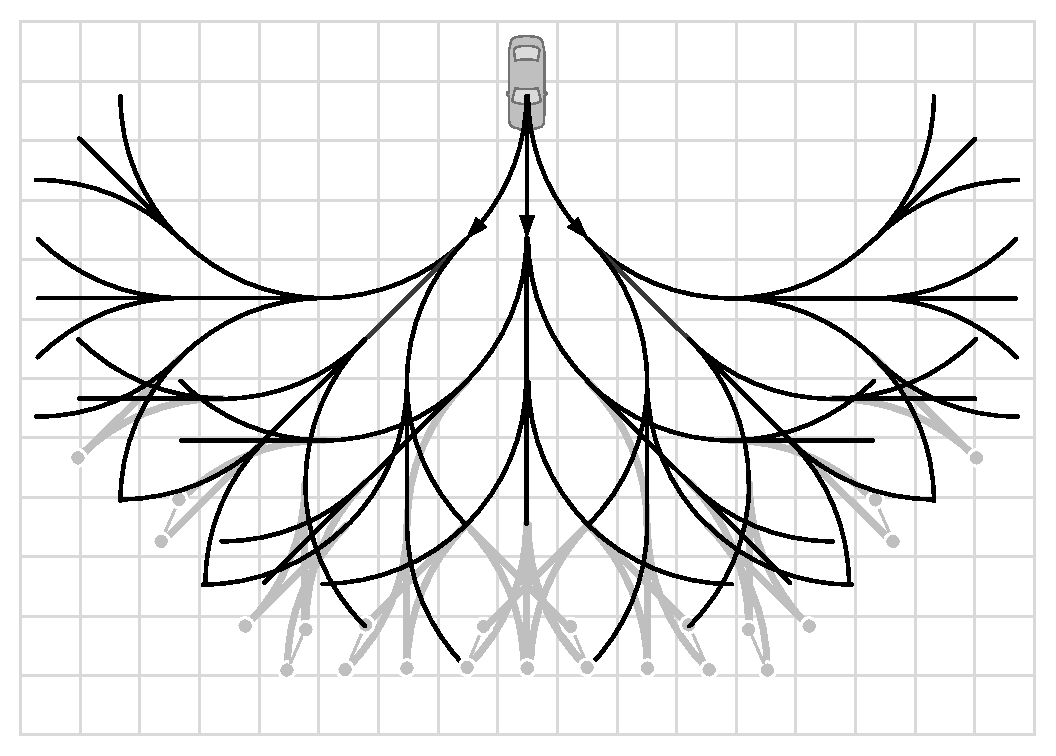
\includegraphics[width=.75\textwidth,clip, trim = 0cm 0cm 0cm 0cm]{7_Pruned_graph.eps}
	\caption[Suchbaum für die Vorwärtsfahrt]{Durch Vorwärtssimulation mit unterschiedlichen Lenkwinkeln entsteht zunächst ein Suchbaum für die Vorwärtsfahrt; Zur Reduktion der Knotenanzahl wird der Graph an Knoten mit einer ähnlichen Position und Ausrichtung geschlossen (betroffene Kanten in Grau); Darstellung basierend auf \cite{Stangl2013}}
	\label{fig:pruning}
\end{figure} 

\subsection{Systematische Ableitung von Heuristiken\index{Heuristik}}
% Zeitvariantes Problem mit festem Zeithorizont -> Value iteration
% Parkplatz: zeitinvariant, variabler Horizont -> A*
Entsprechend Abschn.\,\ref{sec:astern} wird mit dem Einsatz einer geeigneten Heuristik $\hat G^\ast(\bs x)$ das Ziel verfolgt, die A$^\ast$-Suche in die meistversprechende Richtung zu leiten, damit möglichst wenige Knoten expandiert werden. Je geringer $\hat G^\ast(\bs x)$ die wahren Kosten $G^\ast(\bs x)$  bis zum Ziel unterschätzt, desto schneller schreitet die Suche voran. Im Grenzfall $\hat G^\ast(\bs x) = G^\ast(\bs x)$ werden dann genau die zum Ziel führenden Knoten expandiert, was dem Vorgehen bei der Rekonstruktion der optimalen Trajektorie mittels \eqref{equ:navigation_function} in Abschn.\,\ref{sec:wertiteratrion} entspricht. Allerdings setzt die Berechnung der exakten Kosten $G^\ast(\bs x)$ bis zum Ziel die Kenntnis über die optimale Trajektorie voraus und ist damit genau so aufwändig zu bestimmen wie die Lösung des ursprünglichen Problems. Neben einer möglichst geringen Unterschätzung der ausstehenden Kosten zeichnet sich eine gute Heuristik also gleichzeitig durch eine schnelle Berechenbarkeit aus \cite{lavalle2006pa}. \\
Im Unterschied zur Navigation in einem Straßennetz unterschätzt der euklidische Abstand bei Hinderniskonstellationen mit Sackgassen ganz wesentlich die Kosten bis zum Ziel, s.\ Abb.\,\ref{fig:badheuristic} links, und in der unmittelbaren Umgebung zur Zielkonfiguration ist er ebenfalls viel zu optimistisch, da die Fahrzeugausrichtung unberücksichtigt bleibt, s.\ Abb.\,\ref{fig:badheuristic} rechts. Die Folge ist, dass viele Knoten expandiert werden müssen bis die A$^\ast$-Suche den Weg zum Ziel gefunden hat.
\\
\begin{figure}[h]
\centering
\psfrag{1}[bc][bc][1.0]{$d$}
\psfrag{2}[lc][lc][1.0]{$d$}
 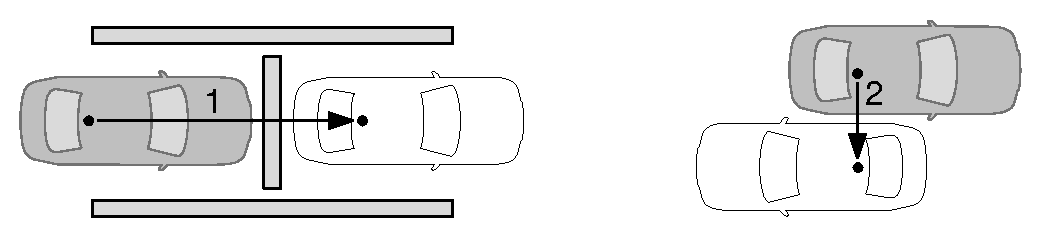
\includegraphics[width=.8\textwidth,clip, trim = 0cm 0cm 0cm 0cm]{7_Nachteile_EuklidischerAbstand.eps}
	\caption[Nachteile des euklidischen Abstands als Heuristik]{Aufgrund der Vernachlässigung von Hindernissen (links) und Unberücksichtigung der Fahrzeugausrichtung (rechts) unterschätzt der euklidische Abstand in vielen Situationen die wahren Kosten bis zum Ziel (weißes Fahrzeug) erheblich \cite{likhachev2009planning}.}
	\label{fig:badheuristic}
\end{figure} 

Ein systematisches Auffinden einer geeigneten Heuristik kann über die gezielte Vereinfachung des Optimierungsproblems erfolgen. Hierbei wird die ursprüngliche Aufgabenstellung darauf untersucht, welche Lockerung (\emph{relaxation}) der Nebenbedingungen und welche Vernachlässigung von Kostenfunktional-Termen zu einer beschleunigten Suche führen. \\
Im konkreten Fall stellt sich das Pfadplanungsproblem beträchtlich einfacher dar, wenn die Hindernisse beiseitegelassen werden, s.\ Abb.\,\ref{fig:heuristics} links (ganz gleich ob sie in den ursprünglichen Nebenbedingungen oder in den ursprünglichen Kosten berücksichtigt werden). Ebenso erheblich wird die Pfadsuche erleichtert, wenn für das Fahrzeug Drehungen im Stand zugelassen werden, s.\ Abb.\,\ref{fig:heuristics} rechts, also die Nicht-Holonomie fallengelassen wird. Die so erhaltenen Heuristiken sind immer optimistisch und damit zulässig. Sie unterschätzen aber die tatsächlich bis zum Ziel anfallenden Kosten in den Situationen, die im Ursprungsproblem durch die jeweils getroffenen Vereinfachungen dominiert werden, sodass sie idealerweise zu kombinieren sind. Da für eine schnelle Suche immer diejenige Heuristik herausgegriffen werden muss, die die Kosten am wenigsten unterschätzt, erfolgt eine optimale Kombination durch  
\begin{align*}
		\hat G^\ast(\bs x) = \max\left( \hat G_1^\ast(\bs x), \, \hat G_2^\ast(\bs x), \ldots \right) \; .
\end{align*}
Der Rechenaufwand der Einzelheuristiken  $\hat G_i^\ast(\bs x)$ kann gering gehalten werden, wenn sich die Lösung der vereinfachten Problemstellung mittels der später in Kap.\,\ref{chap:dynamische_Optimierung_indirekt} dargestellten Methodik geschlossen darstellen lässt. Andernfalls muss vom Ziel aus vorab mittels Dijkstra-Algorithmus für das jeweils vereinfachte Problem solange expandiert werden, bis $\hat G^\ast_i(\bs x)$ für den interessanten Bereich berechnet ist und in der anschließenden Graphensuche des Ursprungsproblems nur noch abgefragt werden muss \cite{dolgov2010path,likhachev2009planning}. Da im Fall der vernachlässigten Hindernisse der Graph unabhängig von der Sensorinformation expandiert werden kann, ist es in dem speziellen Fall sogar möglich, die erforderlichen Berechnungen offline auszuführen, s. \zB \cite{knepper2006high}.
 
\begin{figure}[h]
\centering
\psfrag{1}[rc][rc][1.0]{$\hat {G}^\ast_1(\bs x)$}
\psfrag{2}[rc][rc][1.0]{$\hat {G}^\ast_2(\bs x)$}
\psfrag{3}[rc][rc][1.0]{$\bs x_f$}
\psfrag{4}[rc][rc][1.0]{$\bs x_f$}
 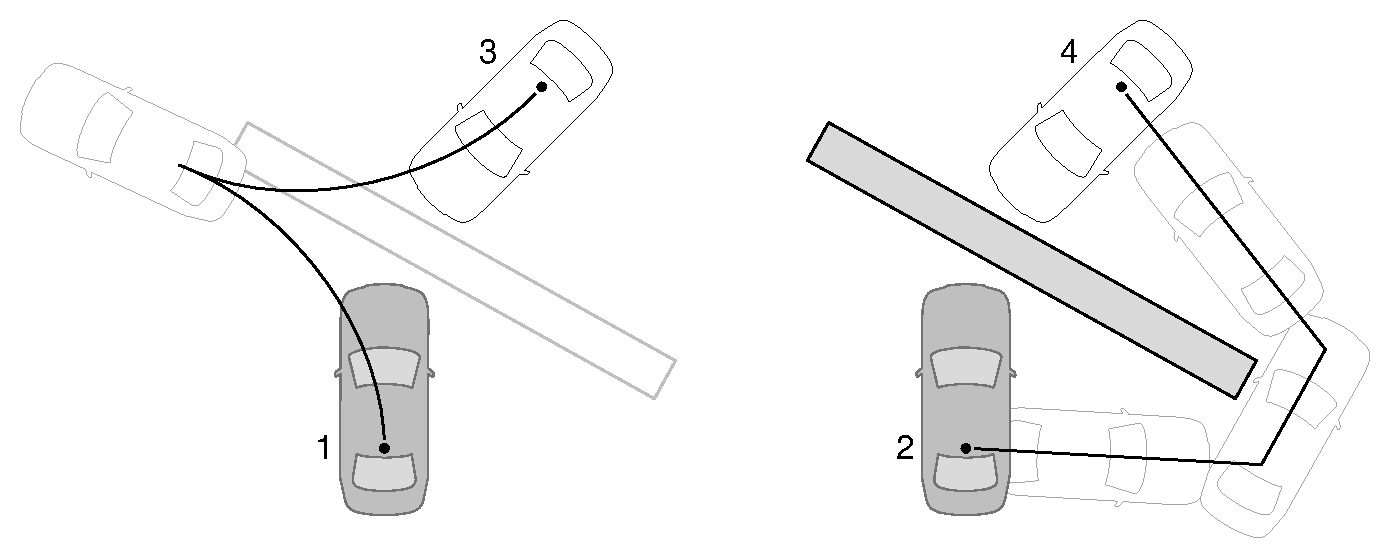
\includegraphics[width=1.\textwidth,clip, trim = 0cm 0cm 0cm 0cm]{7_Vgl_Heuristiken.eps}
	\caption[Gezielte Problemrelaxierung]{Gezielte Relaxierung des Problems führt zu unterschiedlichen Heuristiken, die kombiniert werden können: Ignorieren von Hindernissen (links), Vernachlässigung der Nicht-Holonomie (rechts); Darstellung basierend auf \cite{likhachev2009planning}}
	\label{fig:heuristics}
\end{figure} 

	\section{Bewertung}
	Auch wenn die Methode der Dynamischen Programmierung bislang in der klassischen Regelungstechnik eine untergeordnete Rolle spielt, so ist sie das wichtigste Werkzeug, wenn es darum geht, kombinatorische Optimierungsprobleme zu lösen, wie sie häufig in der Robotik auftreten. Im Bereich der Fahrerassistenzsysteme findet die Dynamische Programmierung auf der Navigations- und Führungsebene Anwendung, was darin begründet ist, dass sie weder eine Startlösung benötigt, noch dass für sie lokale Minima ein Problem darstellen. 
	% Probabilistisch
% Da die Kompromisse wohl überlegt sein müssen, ergeben sich immer problemspezifische Lösungen, wie sie zuvor vorgestellt wurden.
%	Einzig und allein die Methode der dynamischen Programmierung ist dazu geeignet, kombinatorische Probleme der Trajektorienoptimierung zu lösen. 
%Sie benötigt weder eine Startlösung, noch kennt sie lokale Minima. 
Das der Optimierung zugrundeliegende Gütekriterium muss ebenfalls keinen bestimmten Stetigkeitsanforderungen genügen, wie es bei der direkten und indirekten Trajektorienoptimierung der anschließenden Kapitel der Fall ist. \\
Gleichzeitig leidet die Methode der dynamischen Programmierung wie keine andere unter dem \emph{Fluch der Dimensionalität}\index{Fluch der Dimensionalität} \cite{bellmann_DP,foellingeroptimal}, weshalb
die meisten Probleme in geeigneter Weise auf ihr Kernproblem reduziert werden müssen, insbesondere falls die Anwendung eine Echtzeitoptimierung erfordert. Für die Pfadsuche in unstrukturierter Umgebung werden daher \zB als Zustandsgrößen typischerweise nur die Fahrzeugposition $x,y$, die -ausrichtung $\psi$ und die Fahrtrichtung $\nu$  verwendet, nicht aber etwa der Lenkwinkel \cite{dolgov2010path, likhachev2009planning}. Die Folge ist, dass die grobe Lösung des abstrahierten Optimierungsproblems nicht direkt mit Lenk- oder Pedalbewegungen umgesetzt werden kann, da beim Passieren eines jeden Knotens Stellgrößensprünge zu erwarten sind. Die Lösung ist daher noch in einem weiteren Schritt zu verfeinern, indem sie als Startwert für eine nachgelagerte, lokale Optimierung herangezogen wird, s.\ \zB \cite{dolgov2010path}. Alternativ kann sie als zu verfolgende Referenz für eine Methode dienen, die mit ihren Unstetigkeiten zurechtkommt \cite{likhachev2009planning}. 
Für beide Fälle eignet sich die \emph{direkte Optimierungsmethode}, die im nachfolgenden Kapitel erläutert wird.

\cleardoublepage
	
	% Unberücksichtigt:
	%D* als Erweiterung bei dynamischen problemen, die sich nicht allzu sehr in jedme zeitschritt ändern.
	% Interpolation wie bei papageorgiou2012optimierung?
% Nebenbedingungen: Konfiguration space
% + analytical expansions

